\documentclass[conference]{IEEEtran}

\IEEEoverridecommandlockouts
\renewcommand\IEEEkeywordsname{Keywords}

\usepackage[utf8]{inputenc}
\usepackage[T1]{fontenc}
\usepackage[american]{babel}
\usepackage{graphicx}
\usepackage{float}
\usepackage{amsmath, amssymb, exscale}
\usepackage[bookmarks=false]{hyperref}
\usepackage[capitalise]{cleveref}

\hypersetup{
    pdftitle={Case Study 2: Tracking Unmodified Smartphones Using Wi-Fi Monitors}
}

\usepackage{blindtext, xcolor, soulutf8}
\newcommand{\hlgreen}[1]{{\sethlcolor{green}\hl{#1}}}

\def\BibTeX{{\rm B\kern-.05em{\sc i\kern-.025em b}\kern-.08em
    T\kern-.1667em\lower.7ex\hbox{E}\kern-.125emX}}

\makeatletter 
\let\old@ps@headings\ps@headings 
\let\old@ps@IEEEtitlepagestyle\ps@IEEEtitlepagestyle 
\def\confheader#1{% 
% for all pages except the first 
\def\ps@headings{% 
\old@ps@headings% 
\def\@oddhead{\strut\hfill#1\hfill\strut}% 
\def\@evenhead{\strut\hfill#1\hfill\strut}% 
}% 
% for the first page 
\def\ps@IEEEtitlepagestyle{% 
\old@ps@IEEEtitlepagestyle% 
\def\@oddhead{\strut\hfill#1\hfill\strut}% 
\def\@evenhead{\strut\hfill#1\hfill\strut}% 
}% 
\ps@headings% 
} 
\makeatother 

\begin{document}

\title{\huge Tracking Unmodified Smartphones Using Wi-Fi Monitors}

\author{\IEEEauthorblockN{Rui Fernandes (up202103071)}
\IEEEauthorblockA{Department of Computer Science\\Faculty of Sciences of the 
University of Porto}
}

\maketitle

\begin{abstract}
The use of tracking systems based on Wi-Fi transmissions is not new. Such 
systems work by collecting radio frequency signals emitted by smartphones and 
other Wi-Fi enabled devies. Because each packet transmitted contains the MAC 
address of the device that sent it, these can be used to uniquely identify a 
device.

In this report, I provide an overview of a probabilistic method for estimating 
the trajectories of unmodified smartphones based on the transmission of Wi-Fi 
probe messages.\\
\end{abstract}

\begin{IEEEkeywords}
Passive Wi-Fi Monitoring, Trajectory Estimation, Location Privacy
\end{IEEEkeywords}

\section{Introduction}

Location data is central to location based services. However, it is extremely 
sensitive. As a matter of fact, mobility traces are highly unique to an 
individual -- In \cite{deMontjoye2013UniqueIT}, de Montjoye et al. have shown 
that from a dataset containing the location of data belonging to 1.5 million 
individuals, only 4 spatiotemporal points are sufficient to uniquely identify 
95\% of individuals.

In \cite{10.1145/2426656.2426685}, the authors present a system that passively 
tracks unmodified smartphones based on Wi-Fi detections, that offers both a low 
installation cost and requires very little equipment, which is the topic of 
this report.

This report is structured as follows: \cref{sec:problem} describes the problem 
and summarizes the solution proposed by the authors. \cref{sec:analysis} 
provides a critical analysis on the proposed solution. Finally, 
\cref{sec:conclusions} concludes the report.

\section{Problem} \label{sec:problem}

To detect whether Wi-Fi networks are available, smartphones periodically scan 
the Wi-Fi band for access points and listen for beacon frames. By placing Wi-Fi 
monitors in an area of interest, it is possible to detect such transmissions, 
and determine a location trace for every smartphone that passes there, all of 
this without needing to modifying the devices. Essentially, as a smartphone 
moves through an area of interest, it passes by several Wi-Fi monitors that, 
upon each received transmission, report it to a server on a second by second 
basis. The main goal is to then accurately estimate its trajectory.

Broadly speaking, this passive Wi-Fi tracking system has two main components:

\begin{itemize}
    \item \textbf{Wi-Fi monitors:} Each monitor reports the MAC addresses and 
the signal strength of the devices it observed on a second by second basis.
     \item \textbf{Central tracking server:} Processes a set of Wi-Fi 
detections by estimating the most likely spatio-temporal path taken.
\end{itemize}

This approach differs from active Wi-Fi localization in the sense that the 
latter relies on the modification of the device to actively listen for 
stationary APs. Instead, this methods works by placing radio frequency monitors 
in the area of interest.

There exists, however, the possibility that a given smartphone goes undetected, 
which may introduce  \textit{positional ambiguity}. This ambiguity can actually 
rise rather quickly given the fact that a smartphone may not transmit any Wi-Fi 
packets for a period of time. This being said, it is clear that the proposed 
algorithm cannot be a deterministic one due to the stochastic nature of Wi-Fi 
detections.

\subsection{Proposed Solution}

The trajectory estimation problem can formulated using a Hidden Markov model of 
states. As such, the proposed method, which is based on Viterbi’s algorithm, 
takes second by second detections of a moving device as input and estimates the 
most probable path traversed, which can be thought of as sequence of states 
visited in the Hidden Markov model.

Instead of considering the location of each smartphone in each instant, we 
model the distribution of possible locations over a period of time and 
determine the most probable trajectory from this model. In order to reduce the 
possible set of locations, restrictions can be imposed on movements: for 
example, it is assumed that phones travel along a well defined spatial path, 
\textit{e.g.} a network of roads.

In addition, no assumptions are made when it comes to the to path taken. To 
capture this idea, we consider uniform transition probabilities between 
adjacent states. That is, for every segment $i$, $$\forall \ n \in N, \ p(i 
\rightarrow i) = p(i \rightarrow n) = \frac{1}{|N| + 1}$$ where $N$ is the set 
of adjacent segments, and $p(i \rightarrow j)$ the probability associtated to 
the transition from state $i$ to state $j$. In this case, the transition 
probabilities model the behavior at intersections.

Finally, it should also be noted that, since we are only interested in 
detecting moving devices, stationary devices should be filtered out. To do so, 
two simple heuristics are considered. Firstly, if a smartphone has been 
observed for longer than a threshold $\theta$, then it is added to a blacklist. 
On the other hand, to ensure that it is detected when it becomes mobile, if the 
device has not been observed for longer than a threshold $\varepsilon$, then it 
is removed from the blacklist.

\subsection{Limitations}

For one thing, the accuracy of the estimated trajectory is highly dependent on 
the density and geometry of the deployment. In other words, despite being 
suitable for deployment in urban areas, accurate results may not be possible to 
achieve in areas where high-coverage cannot be achieved.

Moreover, the accuracy of the estimate depends mostly on the number of 
dectections of a given smartphone. In order to increase the number of such 
detections, two things can me done: more monitors can be placed on the area of 
interest; however, this option is not always feasible. Other than this, we can 
force smartphones to increase the number of messages transmitted. To do so, the 
authors suggest the following three mechanisms:

\begin{itemize}
    \item Advertise popular access points SSID's.
    \item Emulate access points with SSID's for which a direct probe request is 
    made.
    \item Periodically send RST packets to smartphones, which, in turn, forces 
    them to respond with a CTS packet.
\end{itemize}

Besides, since phones usually transmit Wi-Fi packets at rather long intervals, 
and for short durations of time, it is possible that a smartphone passes 
through an area of interest without being detected. This can also be solved 
with the previous solution of prompting additional transmissions.

Finally, this method is based on the assumption that smartphones travel along a 
well defined path, which means that it is not possible to track free movement. 

\subsection{Results}

Using the previously described mechanisms, in a 12-hour trial using 7 Wi-Fi 
monitors deployed over a 2.8 kilometers road, more than 23,000 different 
devices were observed. In addition, more than 400.000 devices were observed in 
a permanent deployment of 5 nodes during the span of 9 months.

In fact, it was possible to detect a passing smartphone, on average, 69\% of 
the time. Not only this, but this probabilistic method was indeed able to 
accurately estimate the trajectories with mean error of 67 meters  throughout 
the whole trajectory when compared to the GPS ground-truth. Moreover, using 
such Wi-Fi monitors spaced over 400 meters apart, a mean error under 70 meters 
when compared to GPS ground was achieved.

Finally, it should be noted that further post-processing lead to a reduction in 
the mean 

\section{Critical Analysis} \label{sec:analysis}

This works raises a very important question concerning privacy protection -- 
\textit{"How can we safety store the MAC address of each device?"}. Since the 
MAC address present in each packet uniquely identifies a device, they must be 
stored in a secure manner. One solution to this issue would be to perform 
\textit{MAC address anonymization}, in which case we store the hash value of a 
the MAC address instead of the address itself. However, this solution is not 
acceptable as the the mapping between a MAC address and its hash value can be 
reversed. In fact, in \cite{10.1145/2611264.2611266}, it is shown that even for 
the SHA-512 hash function, the re-identification of the MAC addresses can be 
performed in a a matter of minutes. One the other hand, one could use 
\textit{pseudonyms} (temporary unlinkable names), but as it was shown in 
\cite{10.1145/1287853.1287866}, this fails to ensure location privacy due to 
impicit identifiers.  Instead, one could hash the MAC address multiple times, 
store them after encrypting them with a symmetric key or, as suggested in 
\cite{10.1145/2611264.2611266}, use \texttt{bcrypt} or \texttt{scrypt} because 
this functions are difficult to parallelize and specifically designed to 
increase the cost of attacks.

On the other hand, another key question is raised -- \textit{"What can be 
inferred from such mobility traces and how does that affect one's privacy?"}. 
The fact that identifiers such as the MAC address can be linked over time may 
compromise one's privacy. For example, if such monitors are placed over a whole 
city, one could use such mobility traces to infer sensitive information about 
individuals. As shown in \cite{8329504}, \textit{identity attacks} make it 
possible to determine one's gender and education based on their trace, or to 
infer the relationship between two people, for example, if they met on a 
certain day. In addition, \textit{localization attacks} allow us to determine
whether or not someone is at a given place at a give time. This might be 
harmful if we consider, for example, that empty houses may be potential targets 
for theft. To address these issues, one could, for example, apply $k$-anonymity 
or other location privacy-preserving mechanisms in order to anonymize or 
obfuscate such mobility traces (\Cref{fig:k-anonimity}). If applied correctly, 
it would be possible to achieve an acceptable level of utility, which still
allow us to carry out useful tasks (\textit{e.g.} monitoring road traffic).

\begin{figure}[H]
    \centering
    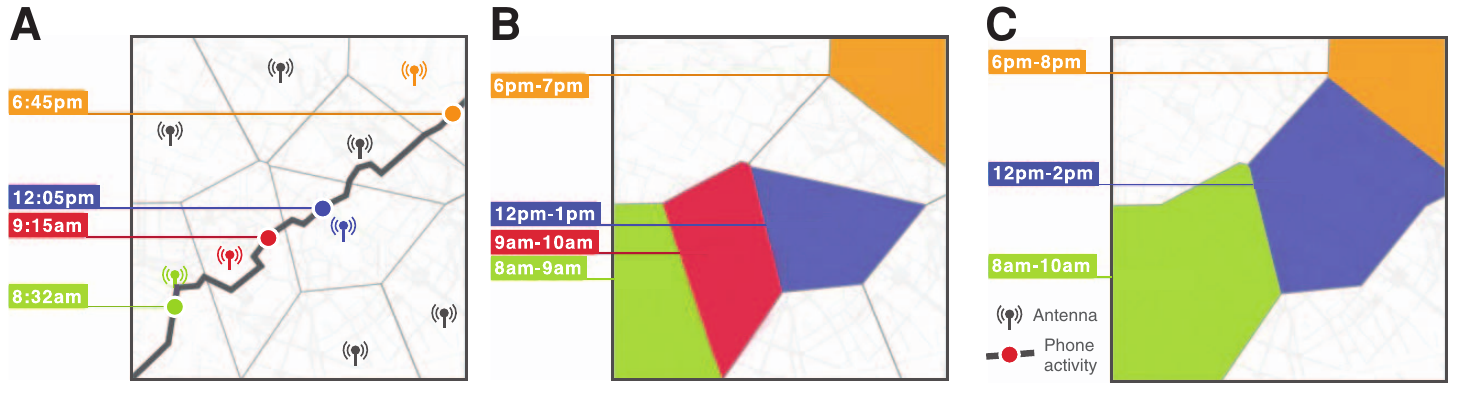
\includegraphics[width=.5\textwidth]{img/k.png}
    \caption{Spatiotemporal obfuscation \cite{deMontjoye2013UniqueIT}}
    \label{fig:k-anonimity}
\end{figure}

\section{Conclusion} \label{sec:conclusions}

It has been shown that using a probabilistic method based on Viterbi’s 
algorithm, a smartphone trajectory can be estimated based on the transmission 
of Wi-Fi probe messages, and relatively accurate results can be achieved. 
Nevertheless, such mechanisms may compromise one's privacy in the sense that 
mobility traces are highly unique to a given individual.

\bibliographystyle{IEEEtran}
\bibliography{refs}

\end{document}
